\documentclass[serif,mathserif,professionalfonts,svgnames]{beamer}
\usepackage{pxfonts}
\usepackage{eulervm}

\usepackage{array}
\usepackage{graphicx}
\usepackage{booktabs}
\usepackage{listings}
\usepackage{fancyvrb}
\usepackage{relsize}

\graphicspath{{Images/}}


\def\E{\mathop{\rm E\,\!}\nolimits}
\def\Var{\mathop{\rm Var}\nolimits}
\def\Pr{\mathop{\rm Pr\,\!}\nolimits}

\providecommand{\abs}[1]{\lvert#1\rvert}
\providecommand{\norm}[1]{\lVert#1\rVert}


\title{Linkage Equilibrium and Disequilibrium}
\author{David H. Alexander}
\date{August 18, 2010}

\mode<presentation>
%\usetheme{Boadilla}


% this is needed for bibliographies to work with beamer
\def\newblock{\hskip .11em plus .33em minus .07em}


\begin{document}
\setlength{\parskip}{10pt plus 1pt minus 1pt}

\maketitle


\begin{frame}{Two-locus dynamics: linkage equilibrium (LE) and disequlibrium (LD)}
  Consider two linked  loci $1$ and $2$.  Let the population frequencies satisfy
  \begin{align*}
    p_A  & =  \Pr(\text{allele } A \text{ at } 1),  \\
    p_B  & =  \Pr(\text{allele } B \text{ at } 2).
  \end{align*}
  \emph{Linkage equilibrium} (LE) between $1$ and $2$ says that the
  alleles an individual has at the two loci are independent, i.e. the
  haplotype $AB$ has population frequency
  \begin{equation*}
    p_{AB} \doteq \Pr(AB) = p_A p_B. 
  \end{equation*}
  \emph{Linkage disequilibrium} (LD) is non-independence between the markers.
\end{frame}


\begin{frame}{Causes of Linkage Disequilibrium (LD)}
\begin{itemize}
\item Linkage equilibrium holds under the following assumptions: a) infinite 
population size, b) no inbreeding, c) random mating, d) no mutation, e) no migration,
and f) no selection.
\item In contrast to HWE, linkage equilibrium is reached over many generations.
\item Disequilibrium is usually attributed to: a) population bottlenecks and founder
effects, b) the recent admixture of two populations, c) selection involving the interaction 
between alleles at different loci, and d) favorable mutations and hitchhiking. 
\end{itemize}
\end{frame}

\begin{frame}{Measures of LD}
  All LD measures assume that loci are biallelic.

  \begin{itemize}
  \item $D$
  \item $D'$
  \item $r^2$
  \end{itemize}

  These LD summary statistics assume \emph{phased} genotype data
  (\emph{haplotypes}), which are hard to come by---requires
  computational \emph{phasing}.
\end{frame}


\begin{frame}{Measures of LD: $D$}
  $$D = D_{AB} \doteq p_{AB}-p_A p_B$$

\begin{itemize}
\item A raw measure of LD
\item $D=0$ indicates linkage equilibrium
\item Problem: range of $D$ varies depending on the allele frequencies of $A$
  and $B$, which makes it hard to interpret nonzero values of $D$
\end{itemize}
\end{frame}

\begin{frame}{Measures of LD: $D'$}
  $$D' = 
  \begin{cases}
    \dfrac{D}{\min\{p_A p_b, p_a p_B \}}, & D \geq 0; \smallskip \\ 
    \dfrac{D}{\min\{p_A p_B, p_a p_b \}}  & D < 0
  \end{cases}
  $$
  \begin{itemize}
  \item A standardized $D$ statistic, $\abs{D'} \leq 1$
  \item $D'=0$ indicates LE, $\abs{D'}=1$ indicates \emph{perfect} LD
  \item Under \emph{perfect} LD, only three of the four possible
    haplotypes occur.
  \end{itemize}
\end{frame}

\begin{frame}{Measures of LD: $r^2$}
  $$r^2 = \frac{D^2}{p_A (1-p_A) p_B (1-p_B)}$$
 \begin{itemize}
  \item Standardized, $0 \leq r^2 \leq 1$
  \item Same as Pearson correlation coefficient between allele
    indicator variables
 \end{itemize}
\end{frame}


\begin{frame}{Example: LD plot}
  Summary plot of pairwise LD statistic ($D'$, $r^2$) 
 \begin{center}
    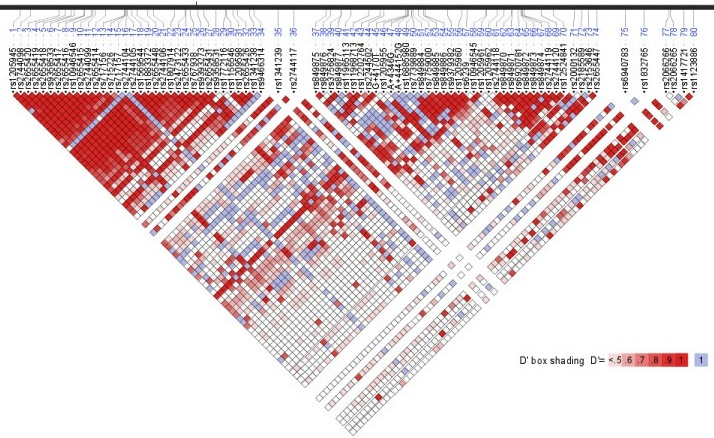
\includegraphics[width=4.5in]{ld-plot.jpg}
  \end{center}
\end{frame}


\begin{frame}{Decay of Linkage Disequilibrium via Recombination}
  \begin{columns}[c]
    \column{2.5in}
    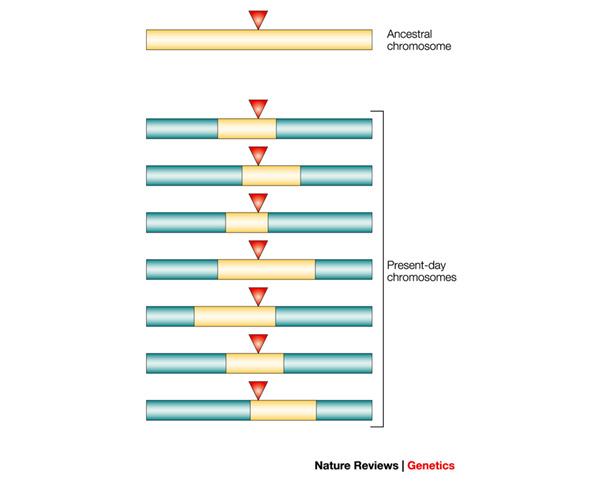
\includegraphics[width=3in]{ancestral-mutation.jpg}
    \column{2in}
    \small
    A new mutation is in perfect LD with all loci on its chromosome. \\[3cm]

    Successive recombinations break up the haplotypes containing the
    mutation. \\[2cm]
  \end{columns}
\end{frame}


\begin{frame}{Decay of LD: the math}
Consider the raw measure of linkage disequilibrium,
$$ D_{AB} = p_{AB}-p_A p_B . $$
Under the equilibrium conditions, at generation $n$ we have
\begin{align*}
  D_{AB}^n & = (1-\theta) D_{AB}^{n-1} \\[0.1cm]
          & = (1-\theta)^n D_{AB}^0 
\end{align*}
so that LD decays geometrically fast, and bigger $\theta
\implies$ faster convergence to LE.  But $\theta \leq 0.5$, so:

Recombination \emph{slowly} breaks up blocks of linkage disequilibrium.
\end{frame}




\begin{frame}{LD is the new normal}
  \begin{itemize}
  \item It used to be that markers were so far apart that LE was the
    norm, and was often assumed. (And there were tests for deviation
    from LE that could be employed to make sure this was a safe
    assumption.)
  \item Now, with very dense marker sets and full sequence data (small
    interlocus $\theta$), LD has become the new norm. Need to take
    care that multimarker analyses do not make independence
    assumptions.
 \end{itemize}
\end{frame}


\begin{frame}{Tests for LD}
  MENDEL offers permutation test procedures to test the null hypothesis of linkage equilibrium.  The test statistic   is the Pearson $\chi^2$ statistic for independence.

\end{frame}



\begin{frame}{Permutation procedure for haplotypes}
  To simulate haplotype under the null hypothesis, we can randomly permute
  data within the columns, shuffling each column separately from the
  others:
  \vspace{-0.4cm}
 \begin{center}
   \framebox{
     \small
      \begin{tabular}{c>{\color{blue}$}c<{$}>{\color{DarkGreen}$}c<{$}}
        & \color{black}\text{Marker 1} & \color{black}\text{Marker 2} \\
        Haplotype 1 & A & b \\                          
        Haplotype 2 & a & B \\
       \vdots & & \\
        Haplotype 2n& A & b \\                          
      \end{tabular}} \bigskip \\
    {\Huge $\: \overset{\text{\normalsize Shuffle}}{\rightsquigarrow} \:$}
    \framebox{
      \small
      \begin{tabular}{c>{\color{blue}$}c<{$}>{\color{DarkGreen}$}c<{$}}
        & \color{black}\text{Marker 1} & \color{black}\text{Marker 2} \\
        Haplotype 1 & a & b \\   
        Haplotype 2 & A & b \\
        \vdots &  &  \\
        Haplotype 2n& A & B \\ 
      \end{tabular}}
  \end{center} \vspace{-0.2cm}
Test for independence of alleles at different markers.
 
\end{frame}

\begin{frame}{Permutation procedure for genotypes}
  Same permutation procedure can be applied even when we don't have
  \emph{phase} information!  Shuffle columns independently, and don't
  break up genotypes.
 \vspace{-0.3cm}
  \begin{center}
    \framebox{\small
      \begin{tabular}{c >{\color{blue}}c >{\color{DarkGreen}}c}
        & \color{black}Marker 1 
        & \color{black}Marker 2 \\
        Multi-genotype 1 & aa       & Bb       \\
        Multi-genotype 2 & Aa       & bb       \\
        $\vdots$         &          &          \\
        Multi-genotype n & aa       & BB       
      \end{tabular}} \bigskip \\
    {\Huge $\: \overset{\text{\normalsize Shuffle}}{\rightsquigarrow} \:$}
    \framebox{\small
      \begin{tabular}{c >{\color{blue}}c >{\color{DarkGreen}}c}
        & \color{black}Marker 1 
        & \color{black}Marker 2 \\
        Multi-genotype 1 & Aa       & BB       \\
        Multi-genotype 2 & aa       & Bb       \\
        $\vdots$         &          &          \\
        Multi-genotype n & aa       & bb       
      \end{tabular}} 
  \end{center} \vspace{-0.2cm}
  Now testing for independence of genotypes, not alleles.
\end{frame}



\begin{frame}{The uses of LD}
  \begin{itemize}
  \item Disease association mapping, i.e. \emph{linkage disequilibrium
      mapping}
  \item Selection mapping---hunting for the signature of natural
    selection
 \end{itemize}
\end{frame}


\begin{frame}{Case-control association (CDCV hypothesis)}
    Case-control association testing is sometimes referred to as a
    method of ``linkage disequilibrium mapping''---hunting for
    genotyped markers that are in LD with putative causal variant.

    \begin{center}
    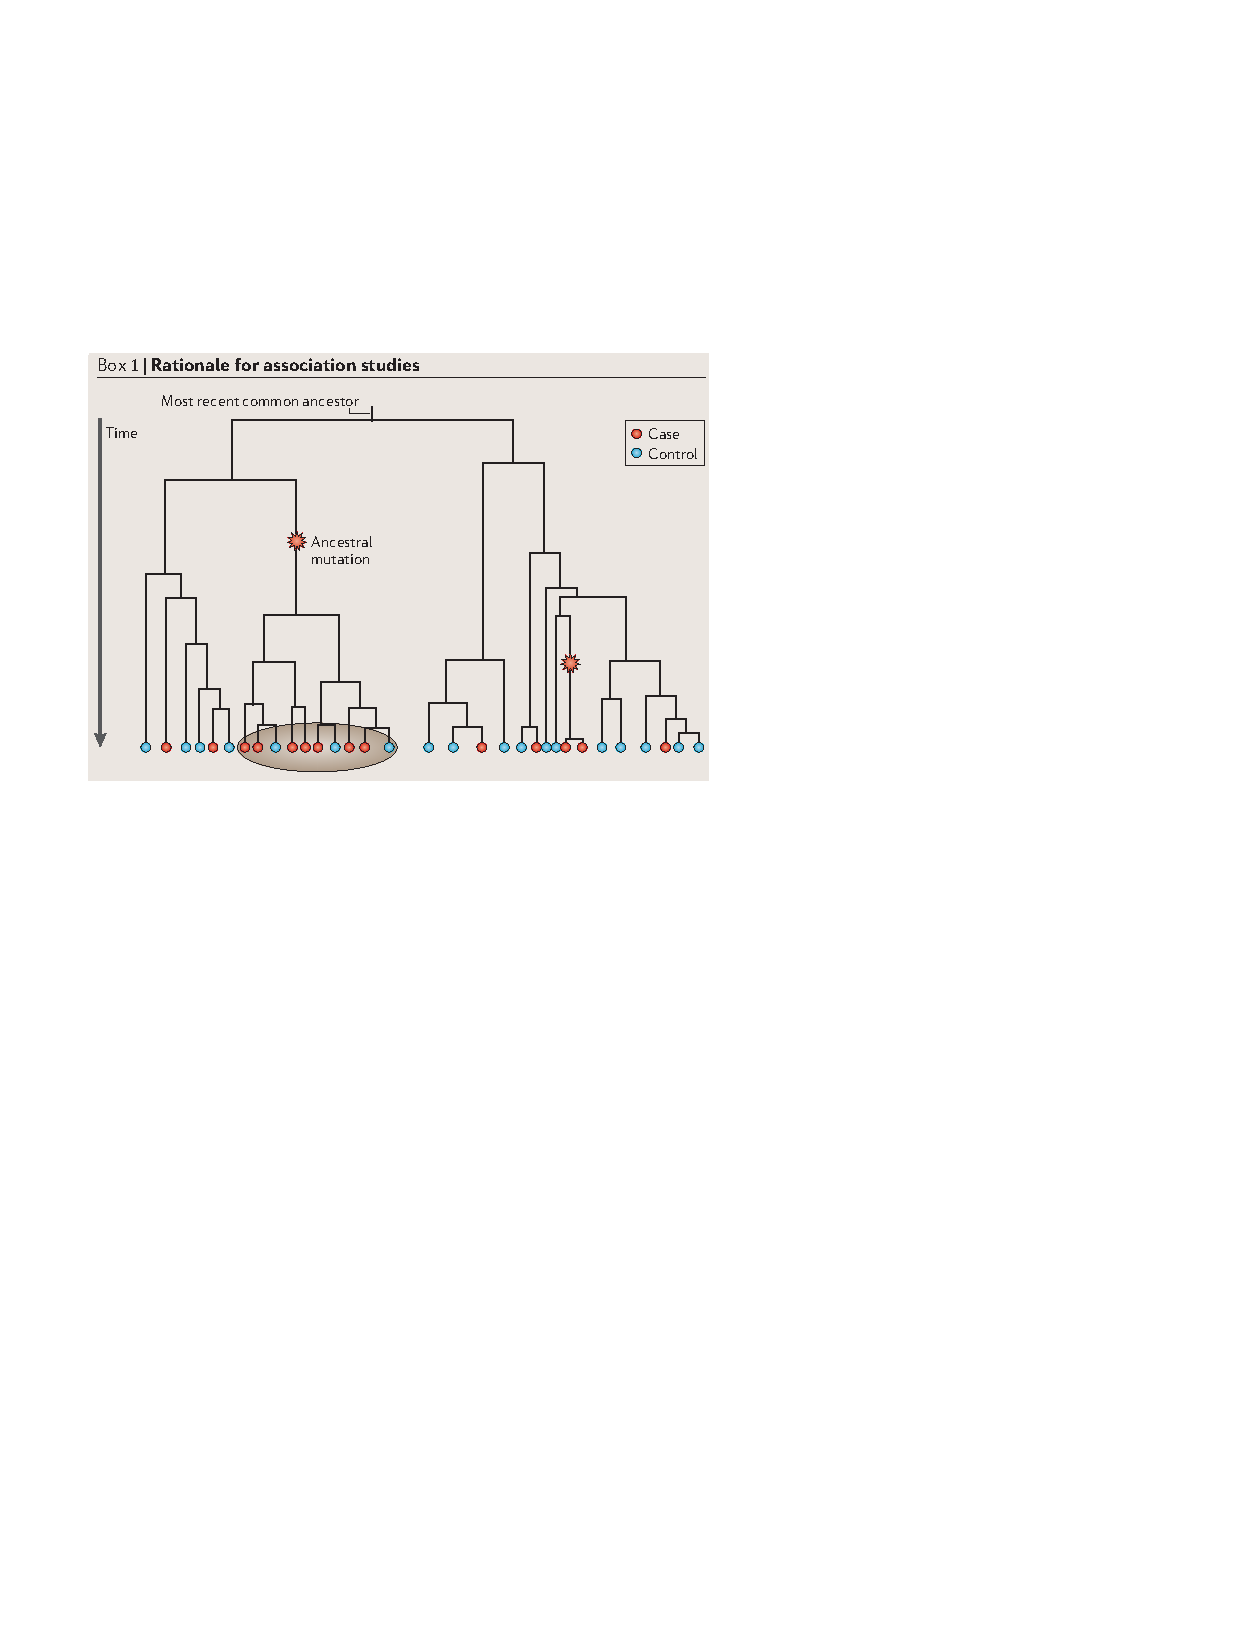
\includegraphics[width=3in]{cdcv.pdf}
    \end{center}
\end{frame}



\begin{frame}{Mapping sites of selection}
 A favorable new mutation will start at frequency $1/2N$ and its
 population frequency will rise towards fixation...

 ...and it will bring its surrounding haplotype with it.  So-called
 ``hitchhiking effect.''

 Population geneticists recently have used patterns of LD to identify
 sites of natural selection.  Tests of neutrality based on ``extended haplotype homozygosity.''
\end{frame}

\begin{frame}{MENDEL Example}
  MENDEL Option 11 ``Genetic Equilibrium'' offers tests for
  Hardy-Weinberg and linkage equilibrium.  

  Try ``Lecture 15c'' example (uses Control11c.in), which tests for pairwise LD in a haplotype dataset

\end{frame}

\begin{frame}[containsverbatim]{MENDEL Results}
%\resizebox{4.5in}{!}{
\begin{Verbatim}[fontsize=\relsize{-2}]
                     DATA TREATED AS HAPLOTYPES

           PAIRWISE TESTS AND STATISTICS FOR LINKAGE EQUILIBRIUM

 FIRST    SECOND    ESTIMATED                 POPULATION  ADJUSTED    DPRIME
 LOCUS    LOCUS      P-VALUE          RANGE      SIZE      CHI-SQ

 Marker1  Marker2   0.0000000                     194     0.80014    0.94360
 Marker1  Marker3   0.0000000                     194     0.40252    0.87799
 Marker1  Marker4   0.0000000                     194     0.55622    0.94085
 Marker1  Marker5   1.0000000                     194     0.00028   -0.19167
 Marker1  Marker6   0.0000000                     194     0.29705    0.87067
 Marker1  Marker7   0.6110000  +/-  0.0097505     194     0.00691   -1.00000
 Marker1  Marker8   0.0000000                     194     0.37464    0.87643
\end{Verbatim}
% }
\end{frame}


\begin{frame}{Recommended reading}
  \nocite{*}
  \bibliography{lecture-15}{}
  \bibliographystyle{unsrt}
\end{frame}



\end{document}